\emph{In problems 1--28, let $U=\{1,2,3,\ldots,10\}$, $A=\{1,3,5,7\}$, $B=\{1,2,3,4\}$, and $C=\{3,4,6,7,9\}$.\\ Find each of the following sets.}

\begin{enumerate}
\item $A^c$ \answer{$\{2,4,6,8,9,10\}$}

\item $B^c$ \answer{$\{5,6,7,8,9,10\}$}

\item $A \cup C$ \answer{$\{1,3,4,5,6,7,9\}$}

\item $A \cap B$ \answer{$\{1,3\}$}

\item $B \cap C$ \answer{$\{3,4\}$}

\item $A \cup B$ \answer{$\{1,2,3,4,5,7\}$}

\item $A \setminus B$ \answer{$\{5,7\}$}

\item $C \setminus A$ \answer{$\{4,6,9\}$}

\item $A^c \cap B^c$ \answer{$\{6,8,9,10\}$}

\item $A^c \cup C$ \answer{$\{2,3,4,6,7,9,10\}$}

\item $B \cup C^c$ \answer{$\{1,2,3,4,5,8,10\}$}

\item $A \cap B^c$ \answer{$\{5,7\}$}

\item $(A \cup C^c)^c$ \answer{$\{4,6,9\}$}

\item $(B^c \cap C)^c$ \answer{$\{1,2,3,4,5,8,10\}$}

\item $(A \cap B)^c$ \answer{$\{2,4,5,6,7,8,9,10\}$}

\item $(B \cup A)^c$ \answer{$\{6,8,9,10\}$}

\item $A \cup \varnothing$ \answer{$\{1,3,5,7\}$}

\item $B \cup \varnothing$ \answer{$\{1,2,3,4\}$}

\item $C \cup \varnothing$ \answer{$\{3,4,6,7,9\}$}

\item $B \cap \varnothing$ \answer{$\varnothing$}

\item $(A \cap B) \cup C$ \answer{$\{1,3,4,6,7,9\}$}

\item $(A \cup C) \cap B$ \answer{$\{1,3,4\}$}

\item $B \cup (A \cap C)$ \answer{$\{1,2,3,4,7\}$}

\item $(A \cap B) \cup (C \cap B)$ \answer{$\{1,3,4\}$}

\item $(B \cup A) \cap (B \cup C)$ \answer{$\{1,2,3,4,7\}$}

\item $(A \cup C)^c \cap B^c$ \answer{$\{6,9\}$}

\item $A \cap B \cap C$ \answer{$\{3\}$}

\item $A \cup B \cup C$ \answer{$\{1,2,3,4,5,6,7,9\}$}
\end{enumerate}
\pagebreak

\emph{In problems 29--40, use the following Venn diagram to find each set.}
\begin{center}
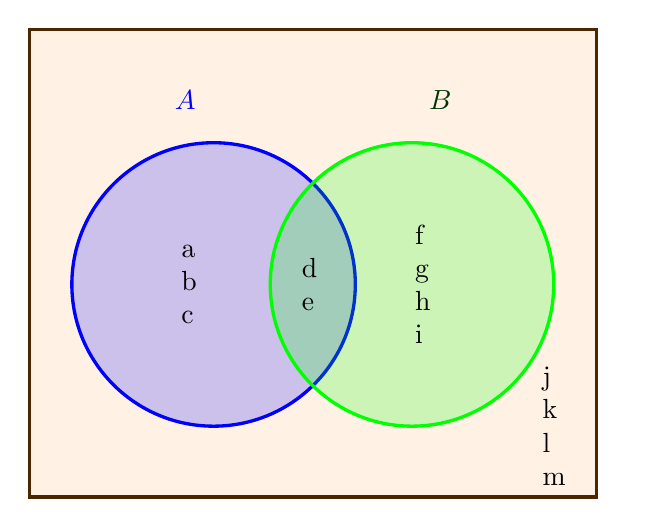
\begin{tikzpicture}[scale=0.9]
  \draw [very thick,color=orange!30!black, fill=orange, fill opacity=0.1] (-4cm,-3cm) rectangle (4cm,3.6cm);

  \draw [very thick,color=blue, fill=blue, fill opacity=0.2] (-1.4,0) circle (2cm);
  \draw [very thick,color=green, fill=green, fill opacity=0.2] (1.4,0) circle (2cm);
  \draw [yshift=2.6cm,xshift=-1.8cm] node {\color{blue} $A$};
  \draw [yshift=2.6cm,xshift=1.8cm] node {\color{green!20!black} $B$};
  
  \draw [yshift=0cm,xshift=-1.3cm] node {\parbox{1cm}{a\\b\\c}};
  \draw [yshift=0cm,xshift=2cm] node {\parbox{1cm}{f\\g\\h\\i}};
  \draw [yshift=0cm,xshift=0.4cm] node {\parbox{1cm}{d\\e}};
  \draw [yshift=-2cm,xshift=3.8cm] node {\parbox{1cm}{j\\k\\l\\m}};
  
\end{tikzpicture}
\end{center}
\begin{enumerate}
\setcounter{enumi}{28}

\item $A^c$ \answer{$\{f,g,h,i,j,k,l,m\}$}

\item $A \cup B$ \answer{$\{a,b,c,d,e,f,g,h,i\}$}

\item $(A \cap B)^c$ \answer{$\{a,b,c,f,g,h,i,j,k,l,m\}$}

\item $A^c \cup B^c$ \answer{$\{a,b,c,f,g,h,i,j,k,l,m\}$}

\item $A \setminus B$ \answer{$\{a,b,c\}$}

\item $B \setminus A$ \answer{$\{f,g,h,i\}$}

\item $A^c \cap B^c$ \answer{$\{j,k,l,m\}$}

\item $(A \cup B)^c$ \answer{$\{j,k,l,m\}$}

\item $U$ \answer{$\{a,b,c,d,e,f,g,h,i,j,k,l,m\}$}

\item $A^c \cup B$ \answer{$\{d,e,f,g,h,i,j,k,l,m\}$}

\item $A \cap B^c$ \answer{$\{a,b,c\}$}

\item $A \setminus U$ \answer{$\varnothing$}
\end{enumerate}